% position an original image/map if useful 
% scale/position manually as desired 

%\begin{pgfonlayer}{shading}
%\node[inner sep=0pt] (Fig8) at (5,5)
%    {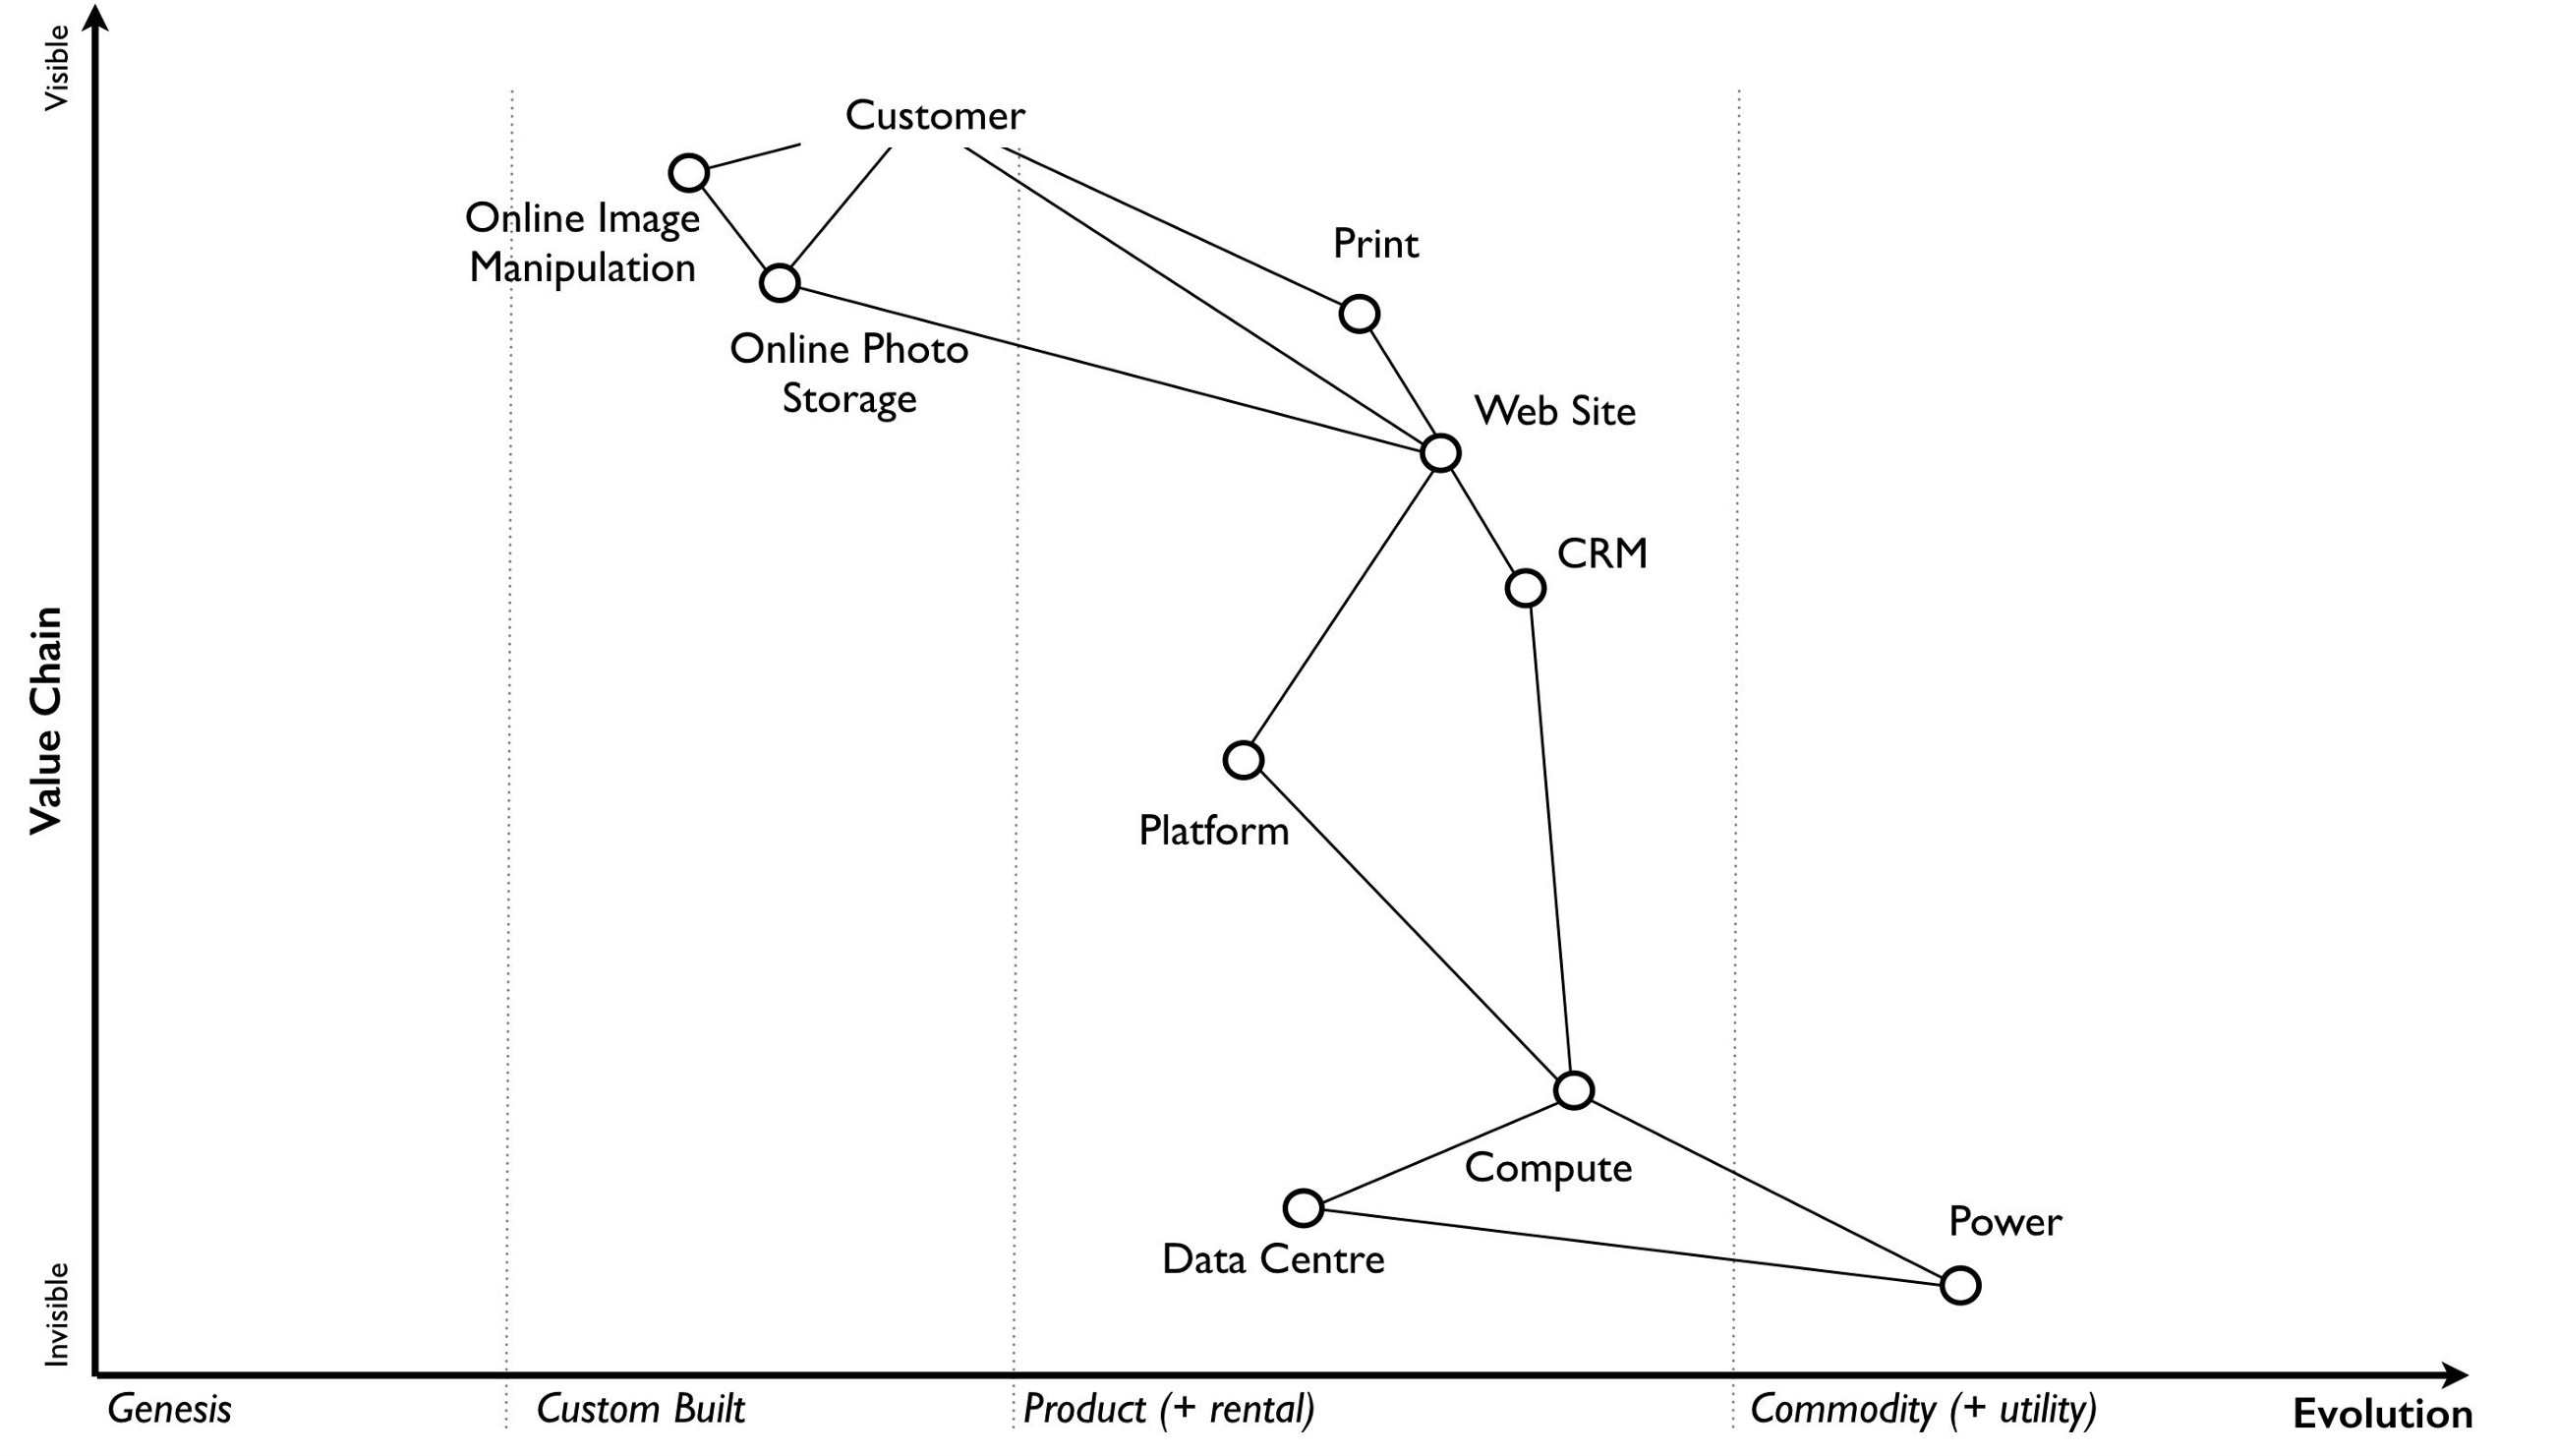
\includegraphics[width=435pt,height=320pt]{images/Fig8_original.jpeg}};
%\end{pgfonlayer}   
    
\begin{pgfonlayer}{map}
% help lines if useful 
%\draw[help lines, step=0.5, color=gray!30, dashed] (0,0) grid (10,10);
 
% x and y axis    
\draw[->,>=angle 60, ultra thick] (0,0)--(10,0) node[right]{$x$};
\node[align=left] at (9.75,-0.3) {Evolution};
    
\draw[->,>=angle 60, ultra thick] (0,0)--(0,10) node[left]{$y$};
\node[align=left,rotate=90] at (-0.3,5) {Value chain};
    
% Genesis
\Text[x=0.4,y=-0.3,color=gray,fontsize=\footnotesize]{\texttt{Genesis}};

% Custom Build
\draw[-, dotted, color=gray, thick] (1.75,-0.4)--(1.75,10);
\Text[x=2.5,y=-0.3,color=gray,fontsize=\footnotesize]{\texttt{Custom Build}};
     
% Product(+rental)
\draw[-, dotted, color=gray, thick] (3.9,-0.4)--(3.9,10);
\Text[x=4.9,y=-0.3,color=gray,fontsize=\footnotesize]{\texttt{Product(+rental)}};
   
% Commodity(+unity)
\draw[-, dotted, color=gray, thick] (6.95,-0.4)--(6.95,10);
\Text[x=8,y=-0.3,color=gray,fontsize=\footnotesize]{\texttt{Commodity(+unity)}}

% Numbering / ticks is useful
% Comment out as desired but you can just omitt whole debug layer 
\begin{pgfonlayer}{debug}
% X-AXIS
\draw[-,color=red, thin] (1,0)--(1,0.1);
\Text[x=1,y=0.2,fontsize=\tiny,color=red]{1};
\draw[-,color=red, thin] (2,0)--(2,0.1);
\Text[x=2,y=0.2,fontsize=\tiny,color=red]{2};
\draw[-,color=red, thin] (3,0)--(3,0.1);
\Text[x=3,y=0.2,fontsize=\tiny,color=red]{3};
\draw[-,color=red, thin] (4,0)--(4,0.1);
\Text[x=4,y=0.2,fontsize=\tiny,color=red]{4};
\draw[-,color=red, thin] (5,0)--(5,0.1);
\Text[x=5,y=0.2,fontsize=\tiny,color=red]{5};
\draw[-,color=red, thin] (6,0)--(6,0.1);
\Text[x=6,y=0.2,fontsize=\tiny,color=red]{6};
\draw[-,color=red, thin] (7,0)--(7,0.1);
\Text[x=7,y=0.2,fontsize=\tiny,color=red]{7};
\draw[-,color=red, thin] (8,0)--(8,0.1);
\Text[x=8,y=0.2,fontsize=\tiny,color=red]{8};
\draw[-,color=red, thin] (9,0)--(9,0.1);
\Text[x=9,y=0.2,fontsize=\tiny,color=red]{9};
\draw[-,color=red, thin] (10,0)--(10,0.1);
\Text[x=10,y=0.2,fontsize=\tiny,color=red]{10};
% Y-AXIS
\draw[-,color=red, thin] (0,1)--(0.1,1);
\Text[x=0.2,y=1,fontsize=\tiny,color=red]{1};
\draw[-,color=red, thin] (0,2)--(0.1,2);
\Text[x=0.2,y=2,fontsize=\tiny,color=red]{2};
\draw[-,color=red, thin] (0,3)--(0.1,3);
\Text[x=0.2,y=3,fontsize=\tiny,color=red]{3};
\draw[-,color=red, thin] (0,4)--(0.1,4);
\Text[x=0.2,y=4,fontsize=\tiny,color=red]{4};
\draw[-,color=red, thin] (0,5)--(0.1,5);
\Text[x=0.2,y=5,fontsize=\tiny,color=red]{5};
\draw[-,color=red, thin] (0,6)--(0.1,6);
\Text[x=0.2,y=6,fontsize=\tiny,color=red]{6};
\draw[-,color=red, thin] (0,6)--(0.1,6);
\Text[x=0.2,y=7,fontsize=\tiny,color=red]{7};
\draw[-,color=red, thin] (0,7)--(0.1,7);
\Text[x=0.2,y=8,fontsize=\tiny,color=red]{8};
\draw[-,color=red, thin] (0,8)--(0.1,8);
\Text[x=0.2,y=9,fontsize=\tiny,color=red]{9};
\draw[-,color=red, thin] (0,9)--(0.1,9);
\Text[x=0.2,y=10,fontsize=\tiny,color=red]{10};
\draw[-,color=red, thin] (0,10)--(0.1,10);
\end{pgfonlayer}


\end{pgfonlayer}